\section{Geometria anatomica e sensibilità della simulazione}
\label{app:anatomy}

La geometria deriva dalla sezione assiale $k=67$ del soggetto \texttt{BraTS20\_Training\_001}. I volumi sono orientati in RAS+ con spacing isotropo di 1 mm; il report registra 202 facce di bordo, area della maschera pari a $17069\,\mathrm{mm}^2$, area della mesh pari a $17068.288\,\mathrm{mm}^2$, Dice 0.998155 e IoU 0.996317. La maschera è un proxy del parenchima: le label BraTS descrivono sottoregioni tumorali e non forniscono una segmentazione della sostanza bianca.

\subsection{Evoluzione temporale e sensibilità alla discretizzazione}

\begin{figure*}[!t]
\centering
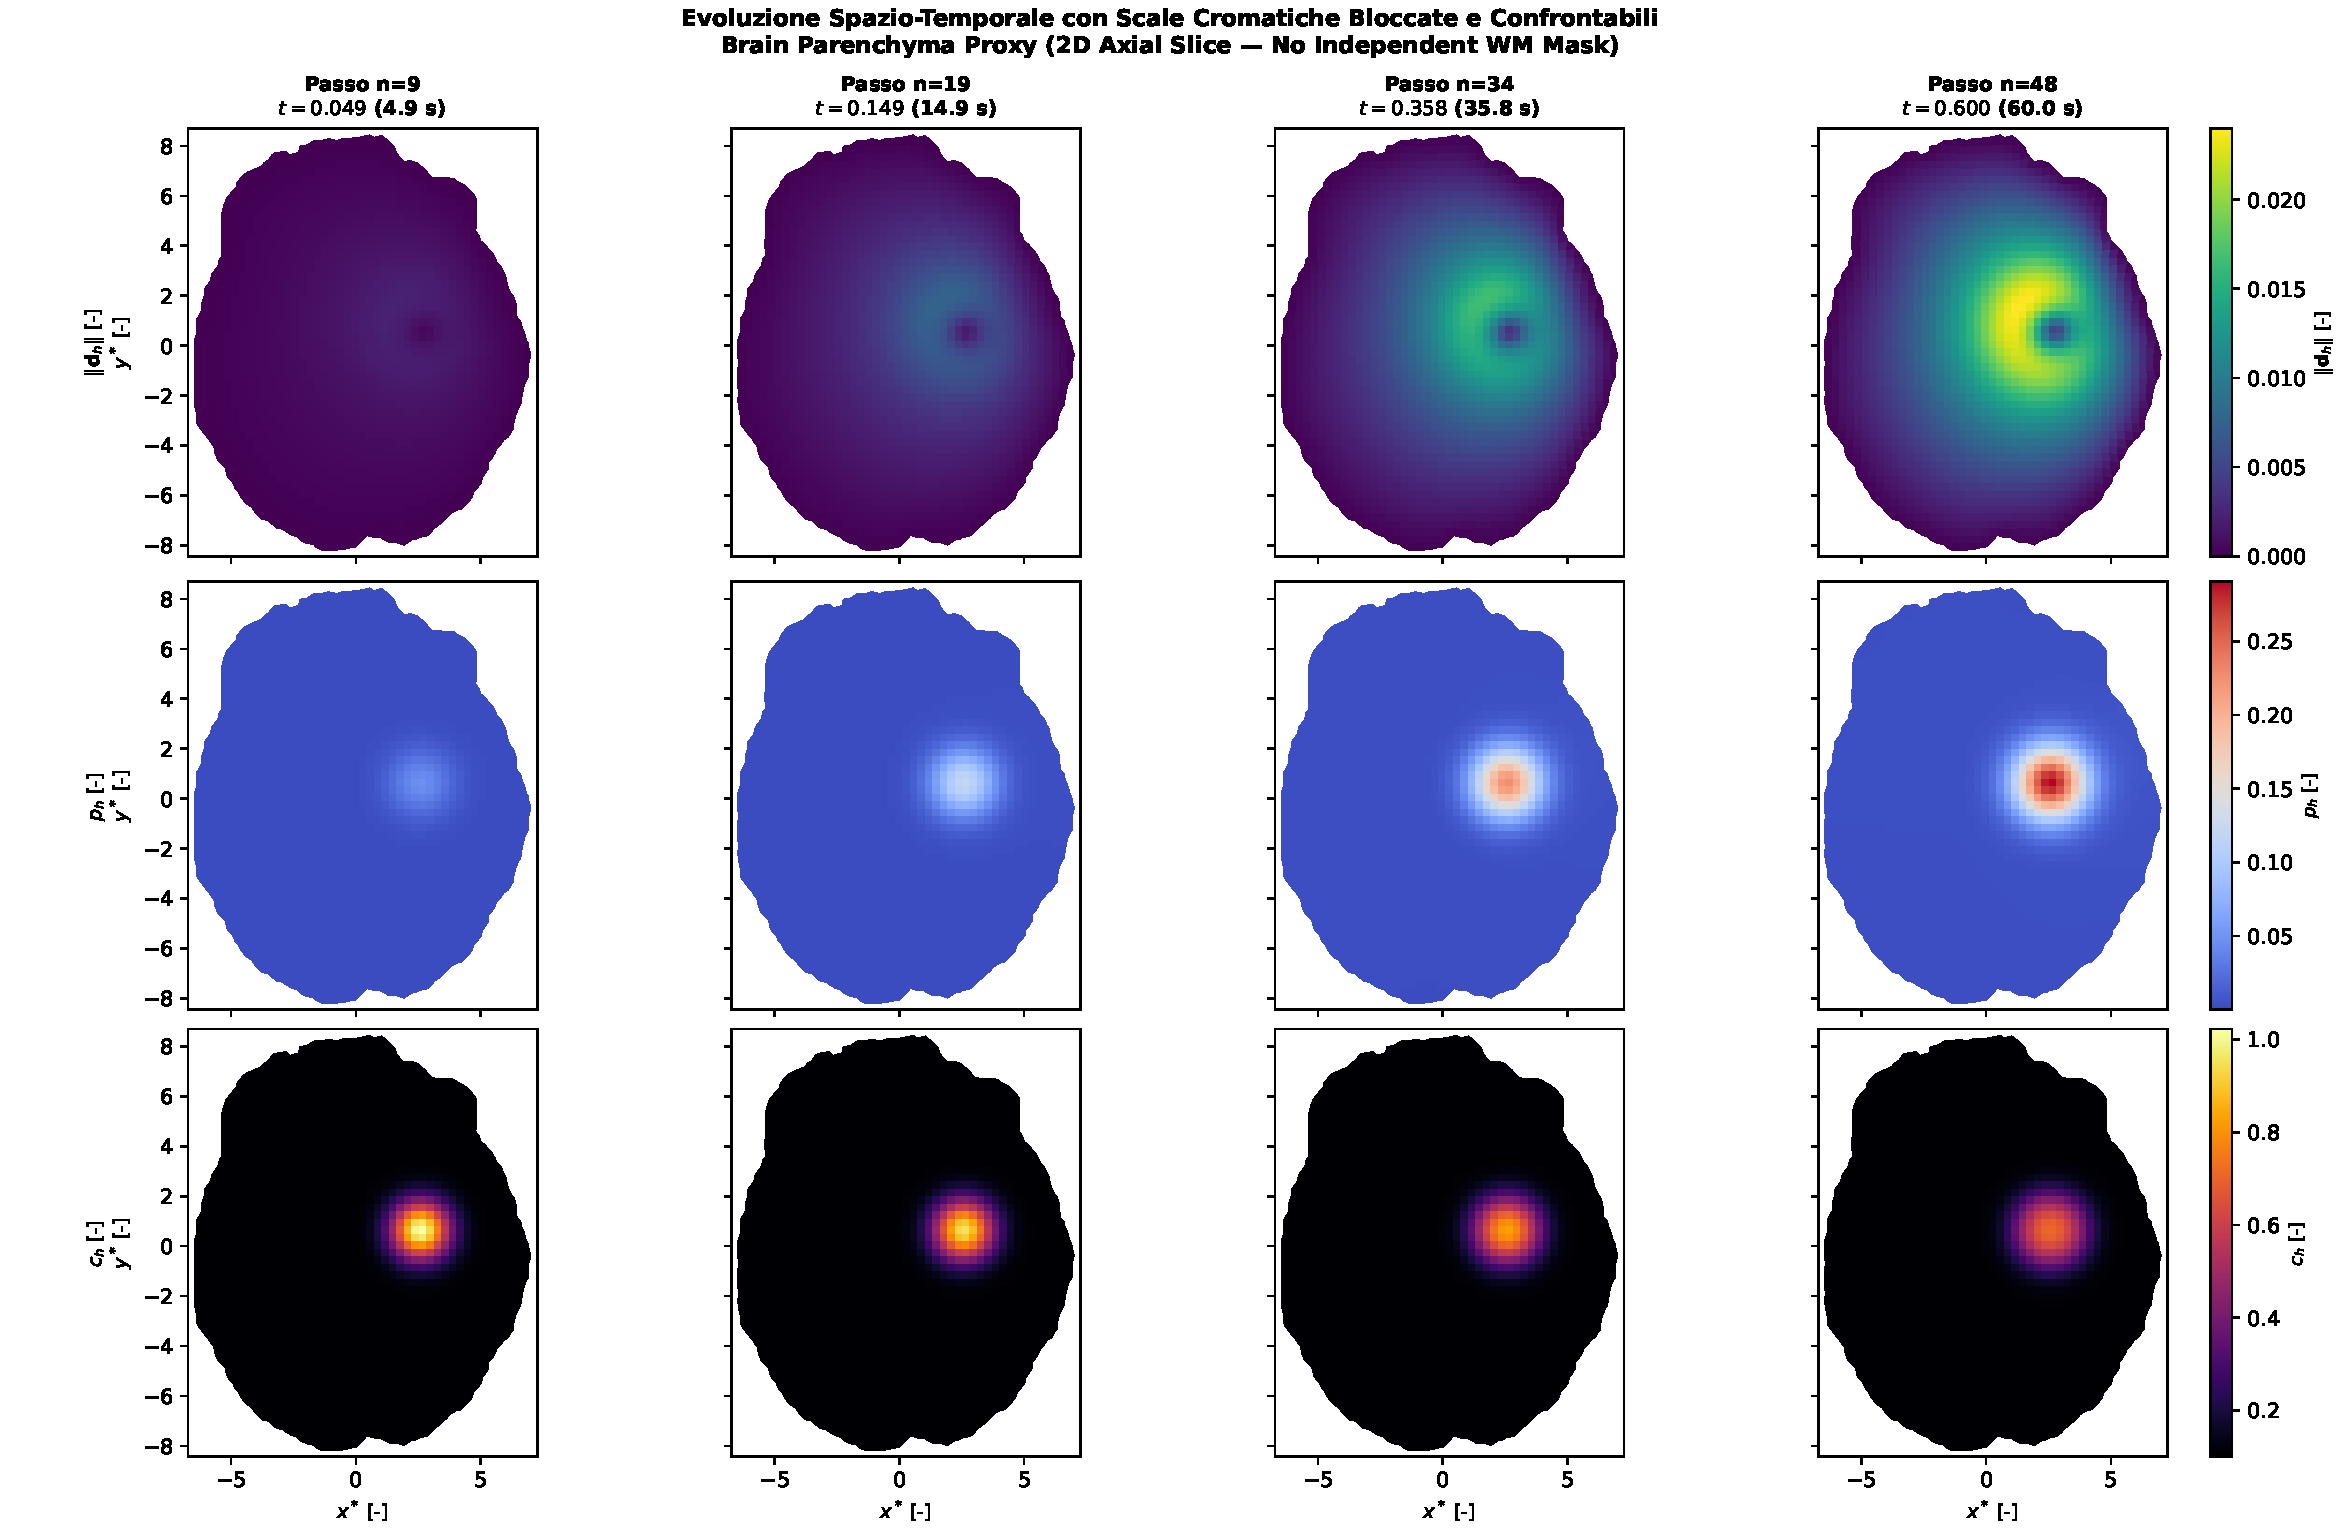
\includegraphics[width=\textwidth]{appendices/figs_07_temporal_evolution_comparable_scales.pdf}
\caption{Evoluzione temporale dei campi sul dominio anatomico. Gli stati sono simulati e dipendono dalle forzanti sintetiche specificate nel testo.}
\label{fig:app-anatomical-time}
\end{figure*}

\begin{figure*}[!t]
\centering
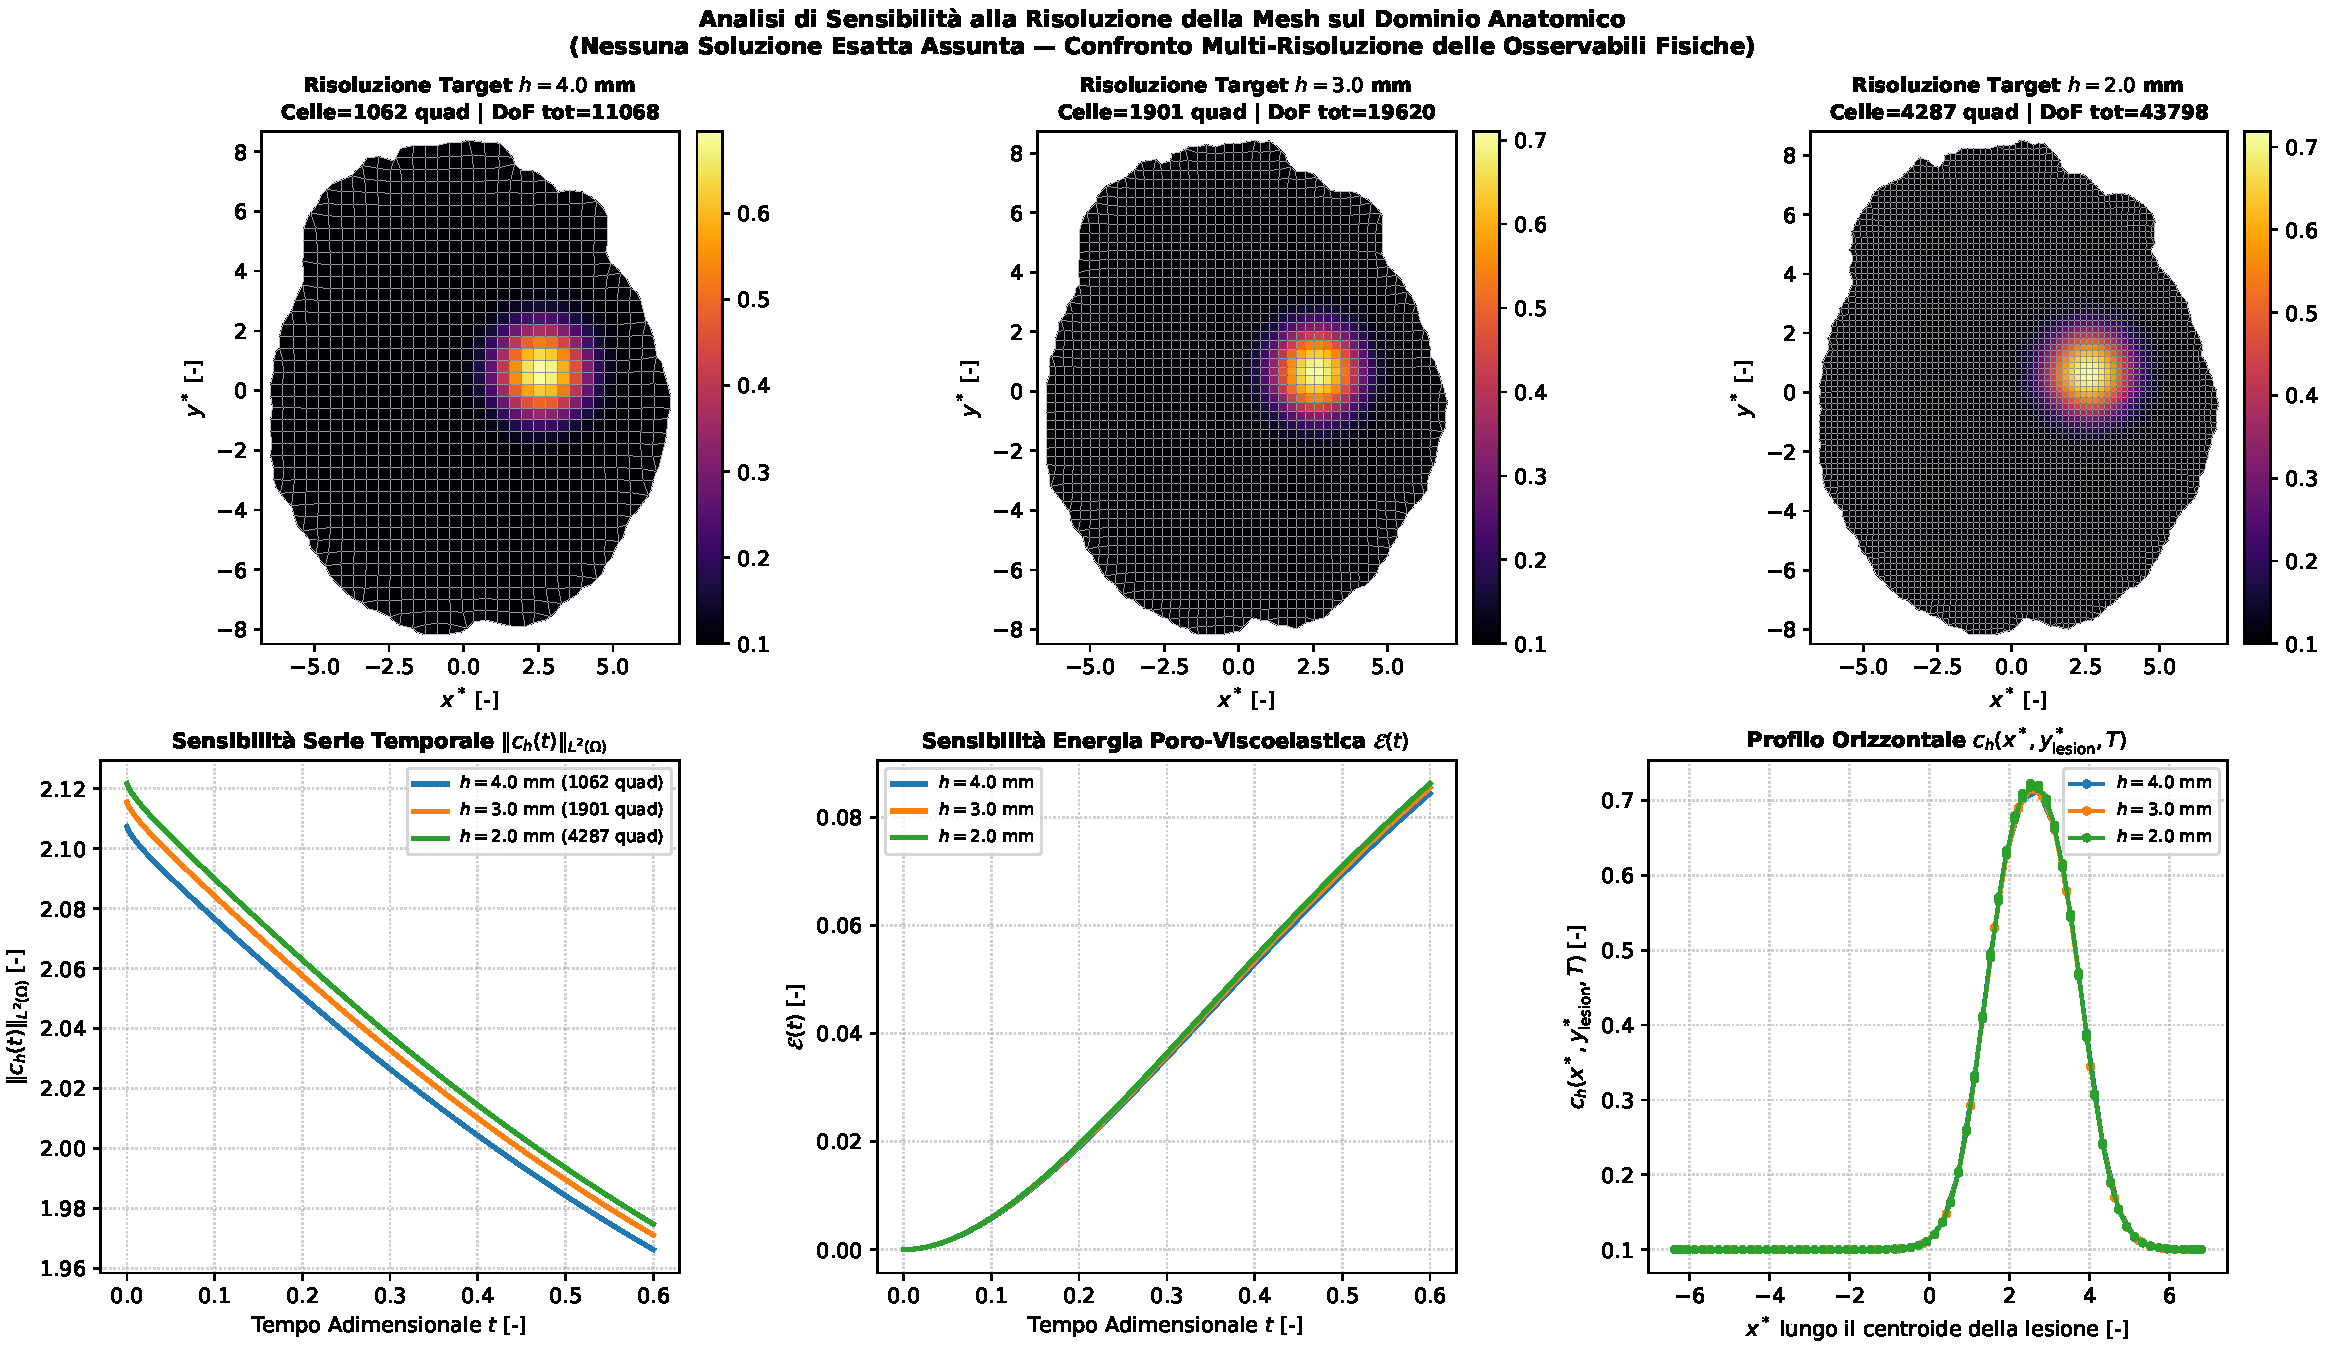
\includegraphics[width=\textwidth]{appendices/figs_08_mesh_resolution_sensitivity.pdf}
\caption{Confronto delle mesh con lati obiettivo pari a 4, 3 e 2 mm. Le differenze rispetto alla mesh più fine sono indicatori di sensibilità alla discretizzazione, non ordini asintotici.}
\label{fig:app-mesh-sensitivity}
\end{figure*}
\FloatBarrier

\subsection{Sensibilità agli ordini frazionari}

\begin{figure*}[!t]
\centering
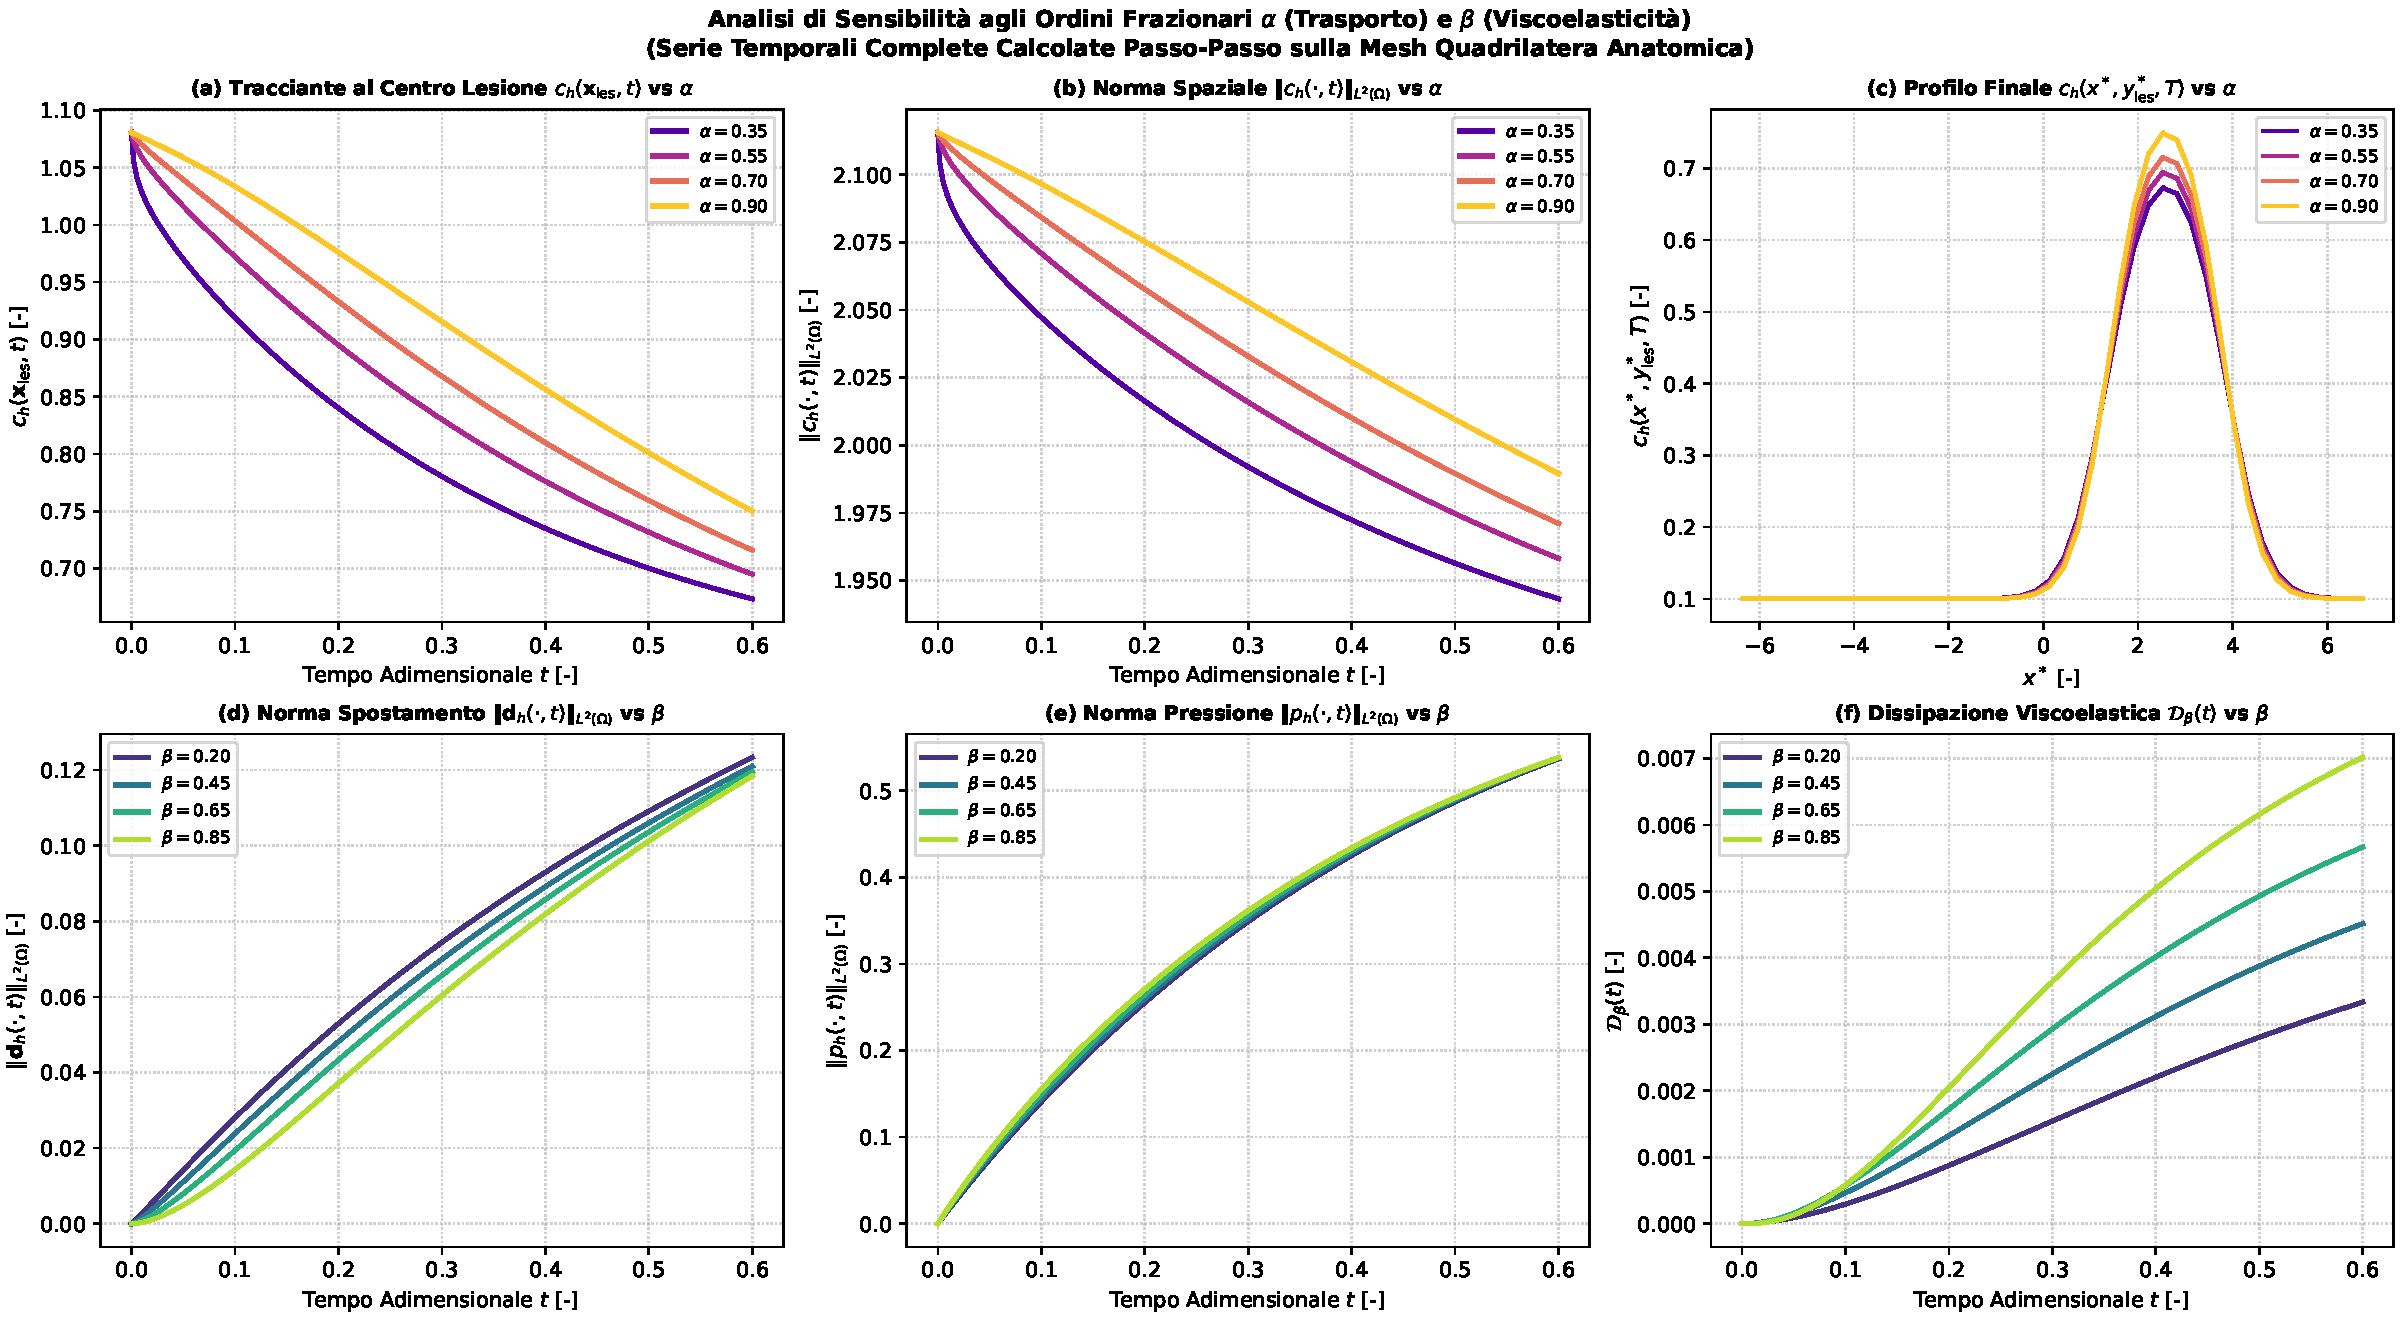
\includegraphics[width=\textwidth]{appendices/figs_09_fractional_parameters_sensitivity.pdf}
\caption{Sensibilità delle quantità di stato a $\alpha$ e $\beta$ nel protocollo anatomico sintetico. Le curve descrivono la risposta del forward model e non costituiscono una prova autonoma di identificabilità.}
\label{fig:app-anatomical-fractional}
\end{figure*}
